\documentclass[../5RO17_TP4.tex]{subfiles}

\begin{document}
\section{Transformation rigide entre nuages de points appariés}
\noindent Lorsqu'on travaille avec des nuages de points, il est parfois necéssaire de déterminer la transformation rigide, c'est-à-dire une combinaison de \textbf{translation} $\mathbf{T}$ et de \textbf{rotation} $\mathbf{R}$, qui relie le même nuage des points dans deux positions différentes dans l'espace.\\

\noindent Plusieur méthodes permettent de trouver cette combinaison de translation et de rotation correspondant à une paire des nuages de points. Ici, nous explorerons la meilleure transformation rigide au sens des moindres carrés.\\

\noindent La transformation recherchée est celle qui minimise l'erreur quadratique totale, donnée par:
\begin{equation}
    f(\mathbf{R}, \mathbf{T}) = \frac{1}{n} \sum_{i=1}^{n} \left[ p_{\text{reference}_i} - (\mathbf{R} \cdot p_{\text{cloud}_i} + \mathbf{T}) \right]^{2}
\end{equation}
Voici les étapes pour appliquer cette méthode:
\begin{enumerate}[noitemsep]
    \item calcul des \textbf{centroïdes} $\bar{p}_{\text{r}}$ et $\bar{p}_{\text{c}}$;
    \begin{equation*}
        \bar{c} = \left(
            \frac{1}{n} \sum_{i=1}^{n} x_{i},\;
            \frac{1}{n} \sum_{i=1}^{n} y_{i},\;
            \frac{1}{n} \sum_{i=1}^{n} z_{i} 
        \right)
    \end{equation*}
    \item centralisation des nuages $q_{\text{r}}$ et $q_{\text{c}}$;
    \begin{equation*}
        q_{\text{r}} = p_{\text{r}} - \bar{p}_{\text{r}}
        \qquad
        q_{\text{c}} = p_{\text{c}} - \bar{p}_{\text{c}}
    \end{equation*}
    \item calcul de la matrice de corrélation $\mathbf{H}$;
    \begin{equation*}
        \mathbf{H} = q_{\text{c}} \cdot q_{\text{r}} ^ {\intercal}
    \end{equation*}
    \item décomposition en valeurs singulières de $\mathbf{H}$;
    \item calcul de la matrice de rotation $\mathbf{R}$ et de translation $\mathbf{T}$;
    \begin{equation*}
        \mathbf{R} = \mathbf{V} \times \mathbf{U}^{\intercal}
        \qquad
        \mathbf{T} = q_{\text{r}} - \mathbf{R} \times q_{\text{c}}
    \end{equation*}
\end{enumerate}

\noindent Ce méthode est implemente ci-dessous:\\

\begin{scriptsize}\mycode
	\begin{lstlisting}[language=Python, caption=\texttt{compute\_rigid\_transformation()}]
def compute_rigid_transformation(
        cloud: np.ndarray[float], reference: np.ndarray[float]
    ) -> list[np.ndarray[float], np.ndarray[float]]:
    '''
    ...
    '''
    # centroides
    centroid_reference = np.mean(reference, axis=1).reshape((3, 1))
    centroid_cloud = np.mean(cloud, axis=1).reshape((3, 1))

    # centering
    centered_reference = reference - centroid_reference
    centered_cloud = cloud - centroid_cloud

    H = centered_cloud.dot(centered_reference.T)

    U, S, V = np.linalg.svd(H)

    R = V.T @ U.T
    T = centroid_reference - R @ centroid_cloud

    return R, T
	\end{lstlisting}
\end{scriptsize}
\begin{remark}
    $\mathbf{R}$ est calculé comme \texttt{R = V.T @ U.T} car \texttt{numpy} retourne la matrice $\mathbf{V}$ transposé.
\end{remark}
En prenant le nuage perturbé comme nuage cible (cloud) et le nuage original comme référence (reference), les résultats obtenus montrent les éléments suivants:
\begin{figure}[H]
    \centering
    \begin{subfigure}[b]{0.325\textwidth}
        \centering
        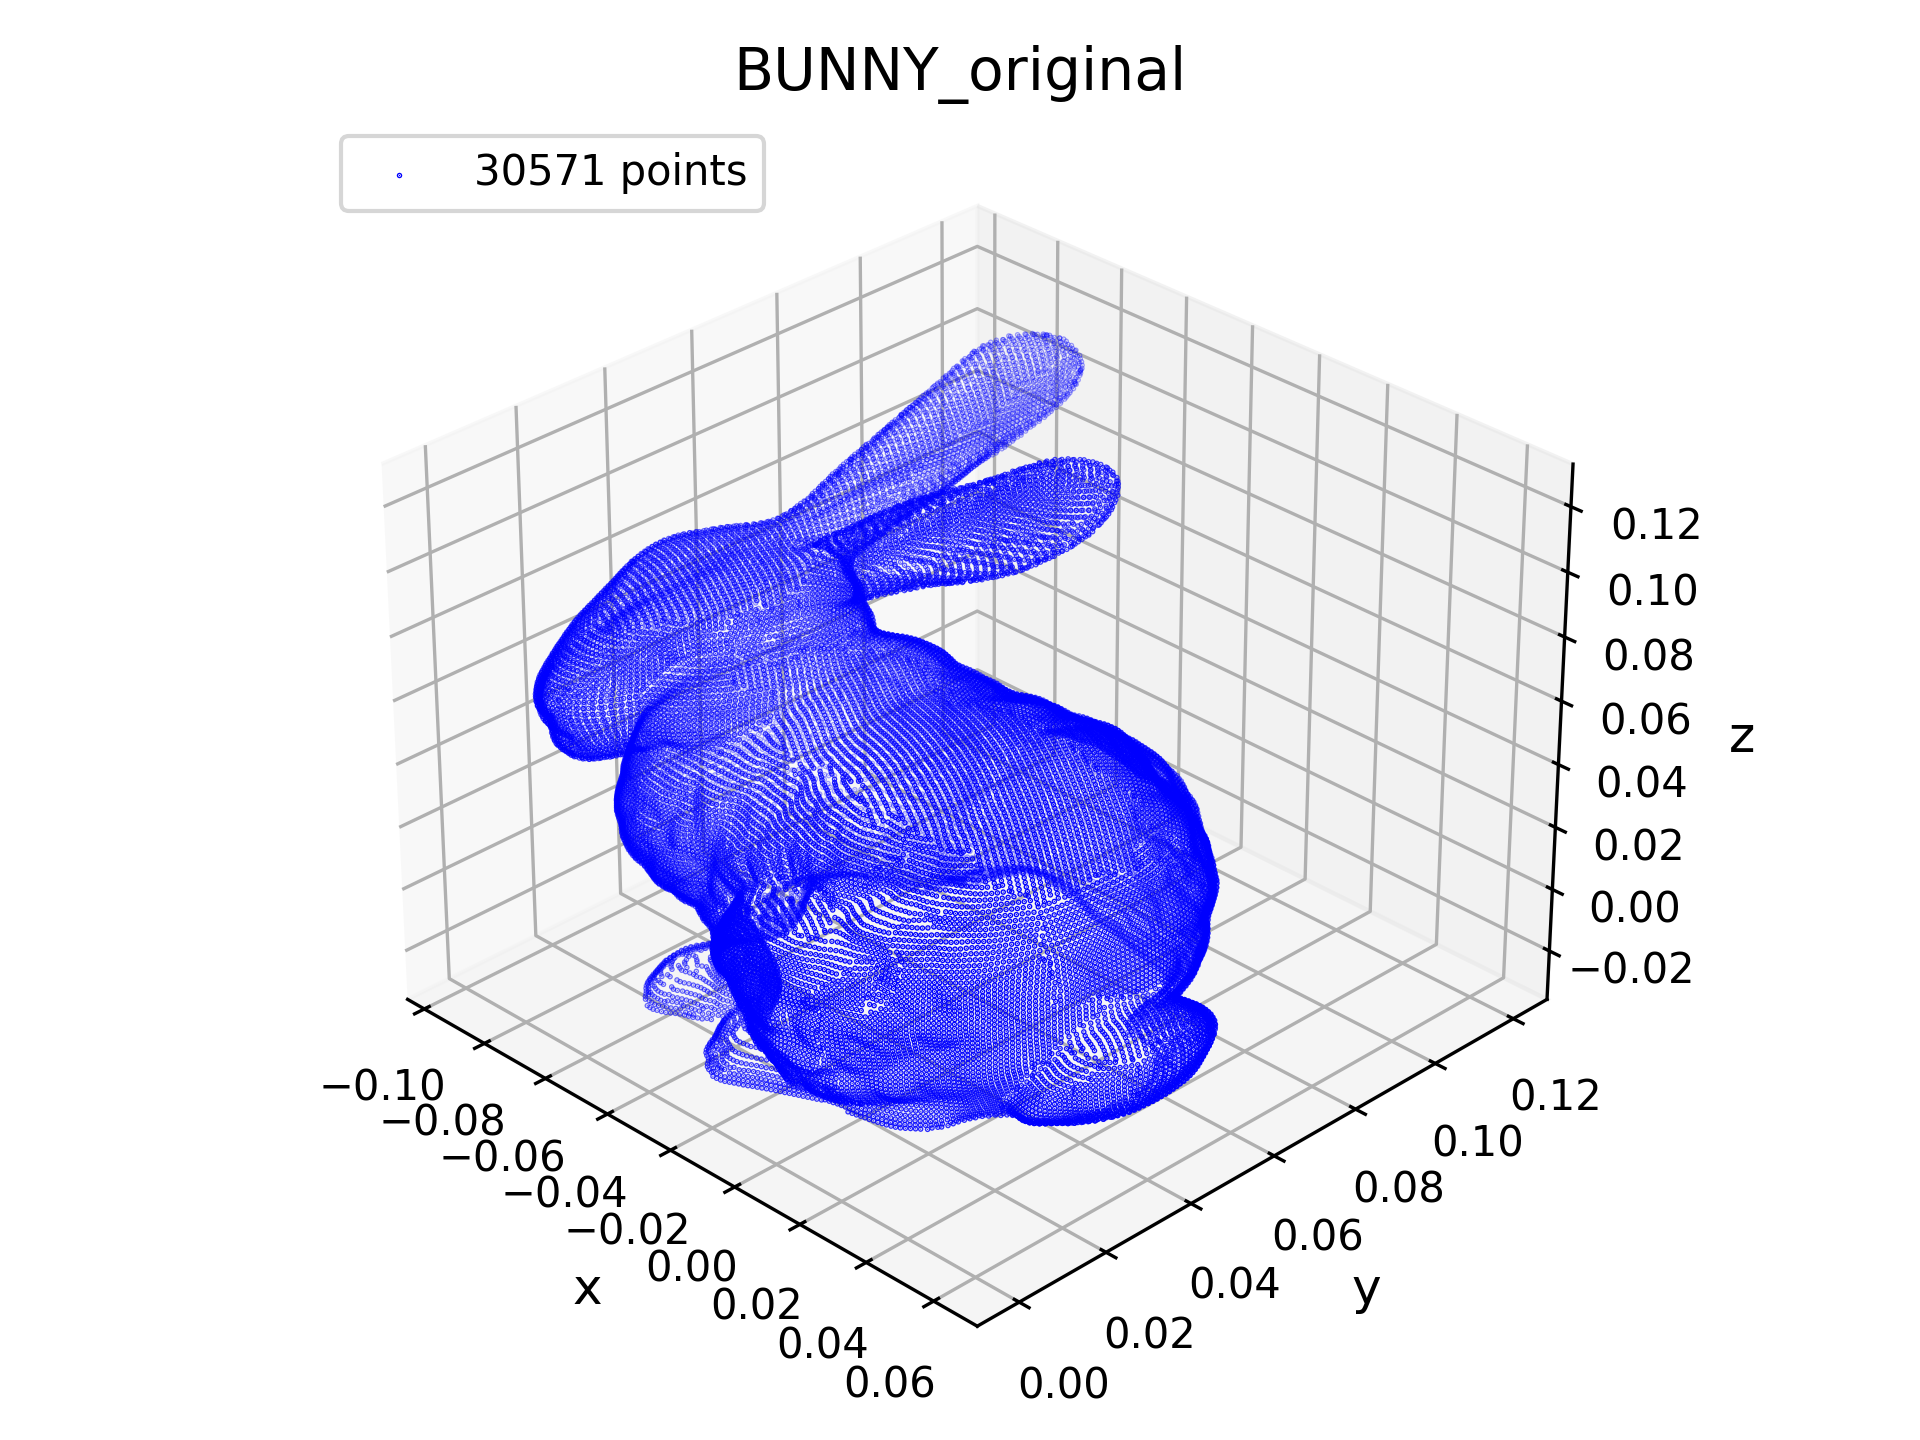
\includegraphics[width=\linewidth]{images/BUNNY_original.png}
        \caption{nuage des points \texttt{reference}}
        \label{}
    \end{subfigure}\hfill
    \begin{subfigure}[b]{0.325\textwidth}
        \centering
        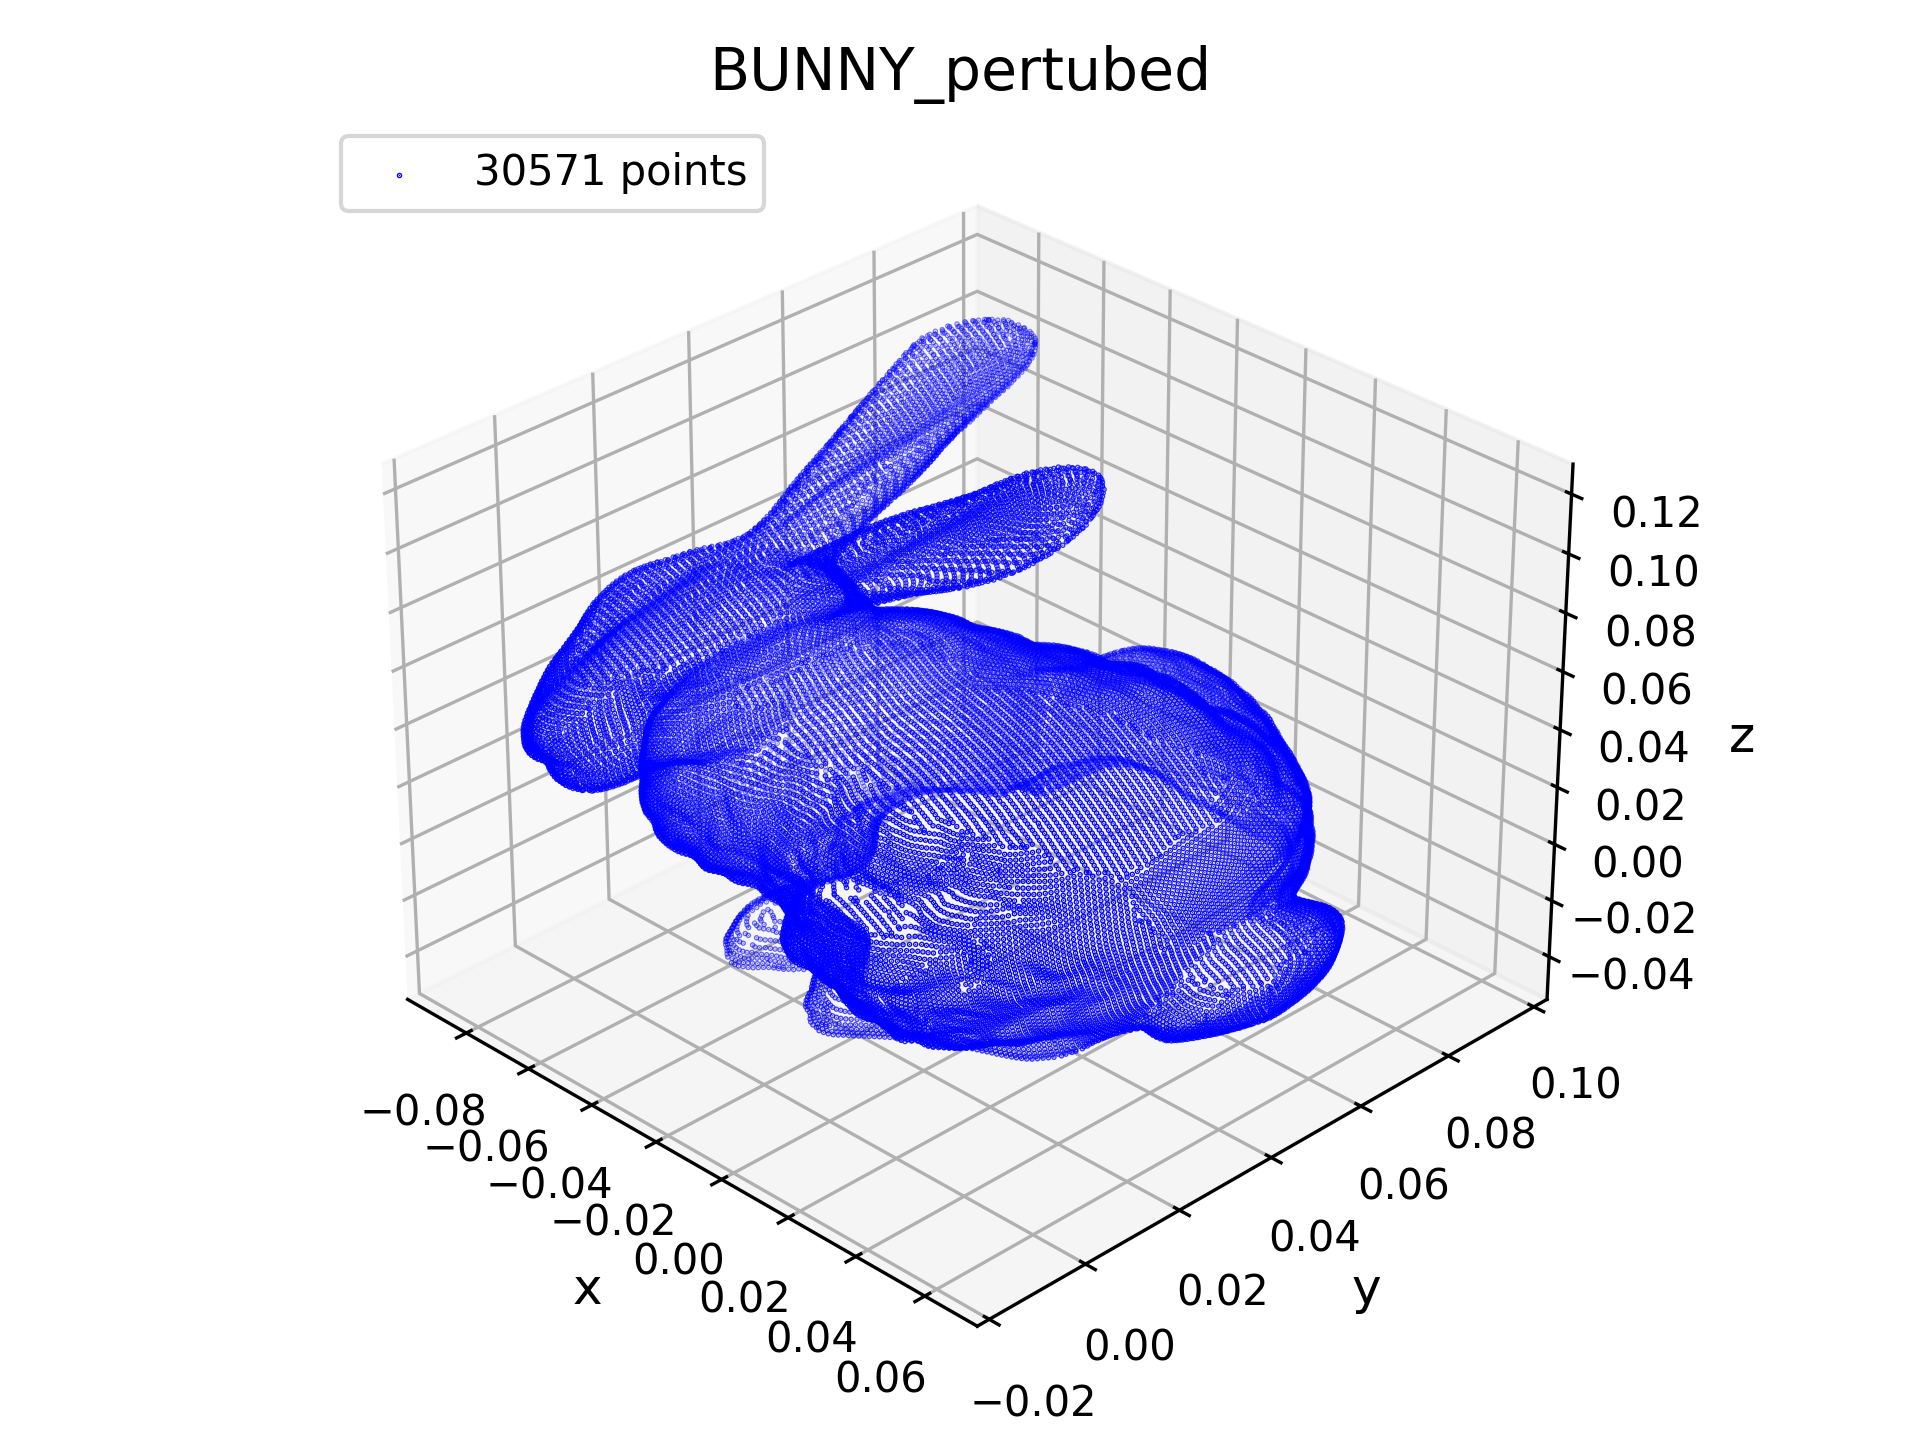
\includegraphics[width=\linewidth]{images/BUNNY_pertubed.png}
        \caption{nuage des points \texttt{cloud}}
        \label{}
    \end{subfigure}\hfill
    \begin{subfigure}[b]{0.325\textwidth}
        \centering
        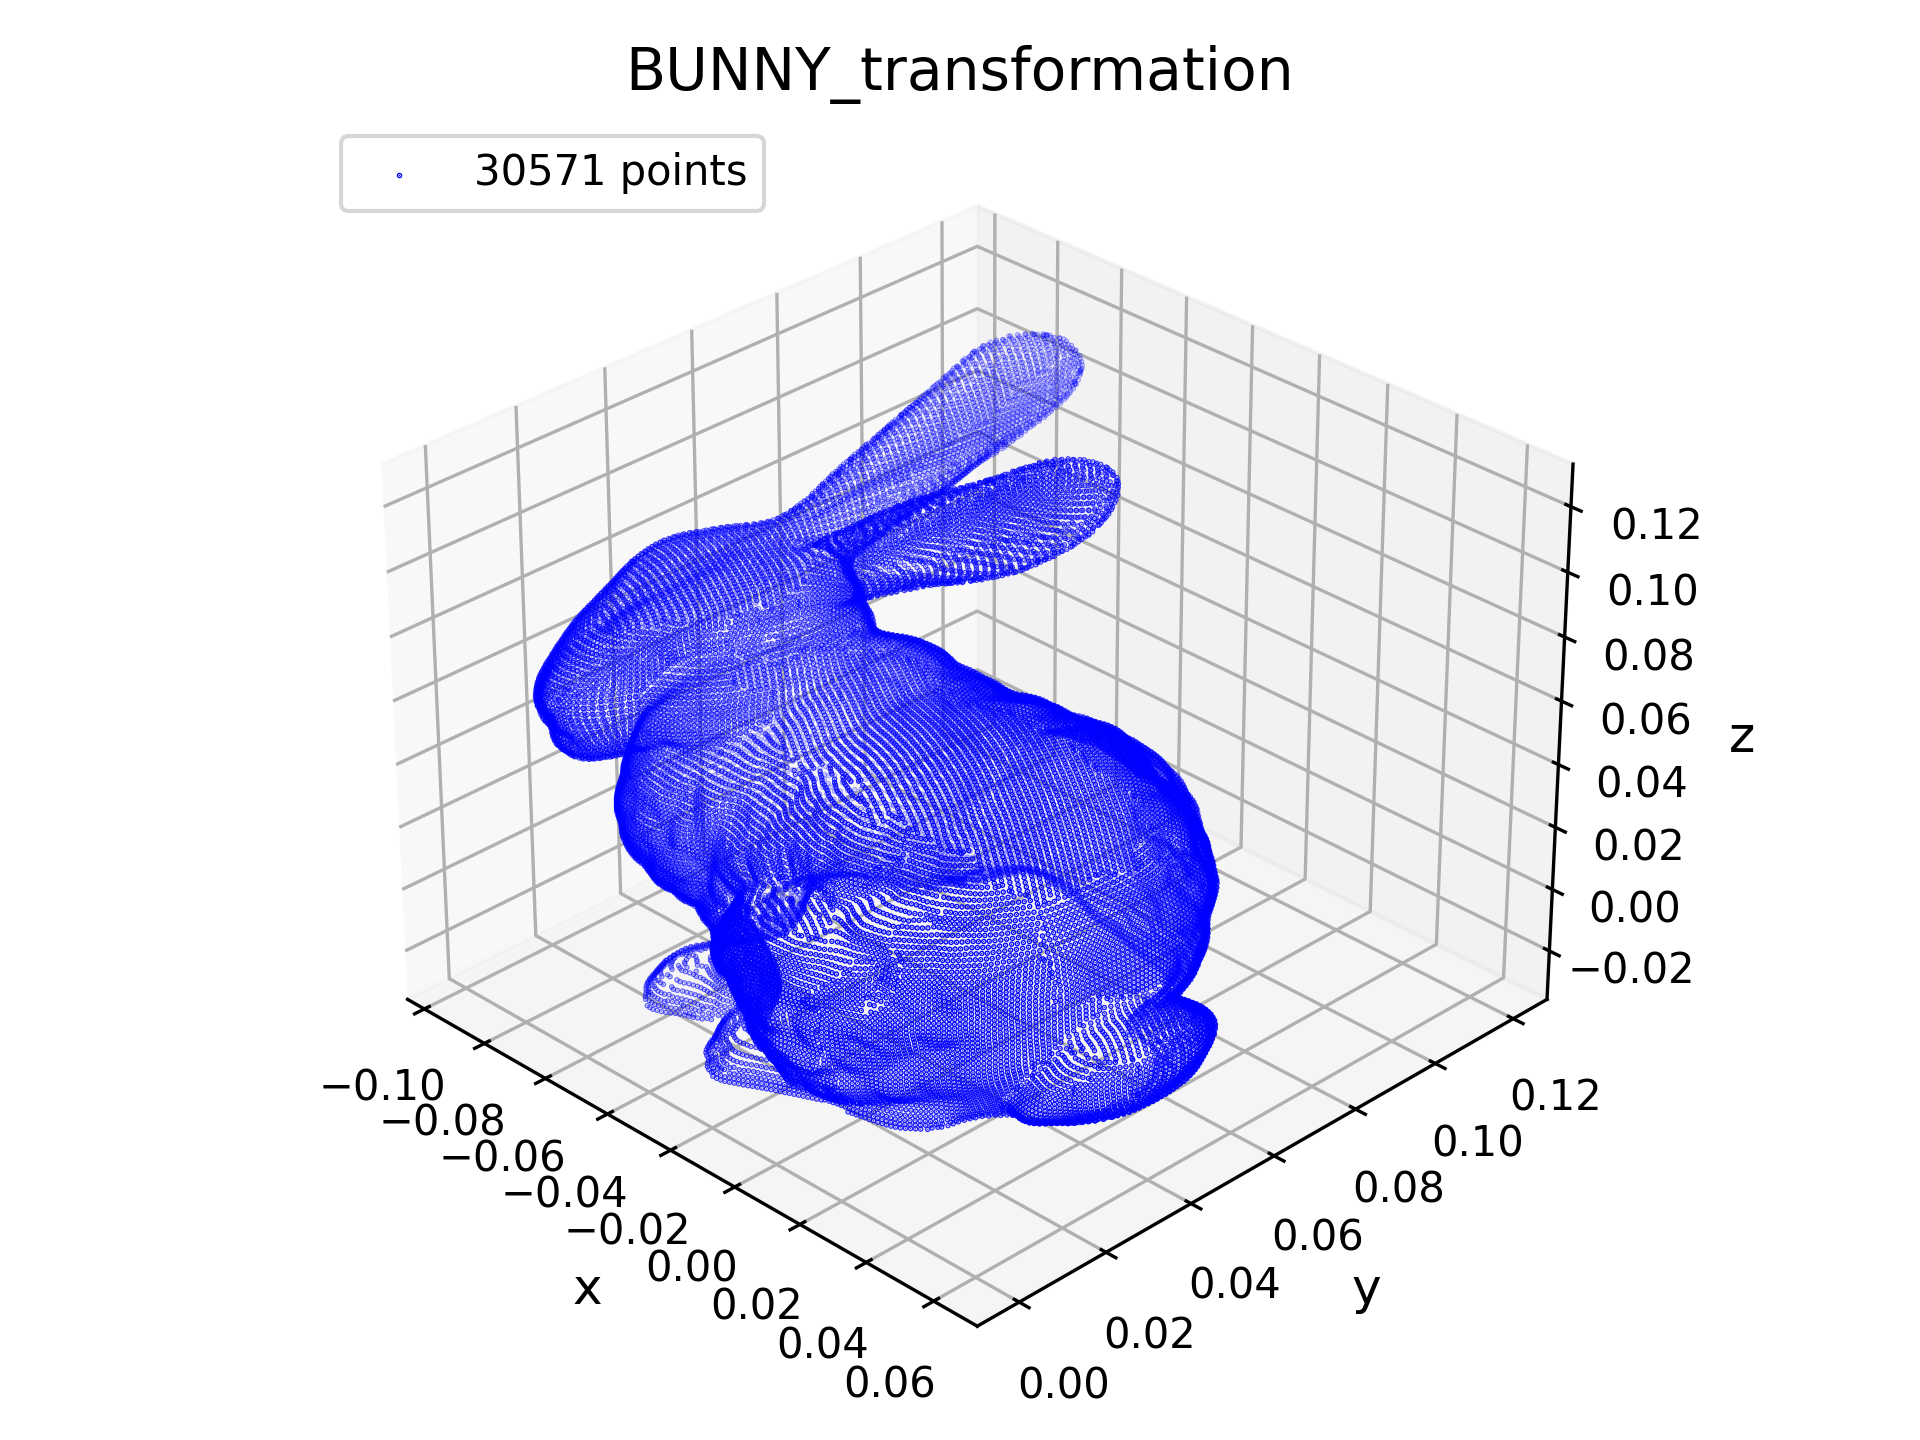
\includegraphics[width=\linewidth]{images/BUNNY_transformation.png}
        \caption{après transformation}
        \label{}
    \end{subfigure}
    \caption{Transformation Rigide pour \texttt{Bunny}}
    \label{}
\end{figure}
\noindent Visuellement, la transformation semble correcte, et pour confirmer ce résultat, l'erreur RMS (Root Mean Square) est calculée comme suit:\\

\begin{scriptsize}\mycode
	\begin{lstlisting}[language=Python, caption=\texttt{RMS()}]
def RMS(points: np.ndarray[float], ref: np.ndarray[float]) -> float:
    return np.sqrt(np.mean(np.sum(np.power(points - ref, 2), axis=0)))
	\end{lstlisting}
\end{scriptsize}
\begin{scriptsize}\mycode
	\begin{lstlisting}[language=Python, caption=\text{Execution \texttt{main()}}]
# print overall results
print('Average RMS between points :')
print(f'RMS pertubed = {RMS(pertubed_cloud, original_cloud):e}')
print(f'RMS returned = {RMS(returned_cloud, original_cloud):e}')
	\end{lstlisting}
\end{scriptsize}
\begin{scriptsize}\mycode
	\begin{lstlisting}[language=Bash]
Average RMS between points :
RMS pertubed = 1.924168e-02
RMS returned = 8.670412e-09
	\end{lstlisting}
\end{scriptsize}

\noindent Comme on peut le voir, l'erreur RMS est très proche de zéro, ce qui indique que la transformation a été correctement exécutée. Cela confirme que le nuage de points perturbé est bien aligné avec le nuage de référence, validant ainsi la précision de la transformation appliquée.

\begin{remark}
    À titre de curiosité, la matrice de transformation et la matrice de rotation obtenues sont présentées ci-dessous:
    \begin{equation}
        T = \begin{bmatrix}
            -0.00902678\\
            +0.00118171\\
            +0.02020558\\
        \end{bmatrix}
        \qquad
        R = \begin{bmatrix}
            +0.99175130 & +0.12809384 & -0.00461713\\
            -0.12423729 & +0.96950660 & +0.21123928\\
            +0.03153481 & -0.20892318 & +0.97742350\\
        \end{bmatrix}
    \end{equation}
\end{remark}
\end{document}
